\chapter{Desarrollo de Aplicaciones}

En este capítulo se hablará sobre las diferentes librerías que se han realizado en este proyecto, explicando detalladamente la estructura de cada una de ellas.

Primeramente se explicará J-OSMClient, que es el cliente programado en Java para comunicarse con la REST API que exporta OSM.

Seguidamente se hablará de J-ONOSClient, que es el cliente encargado de comunicarse con la REST API de ONOS, y de J-OpenStack Client, que se encarga de comunicarse con la REST API de OpenStack.

Por último, se hará especial énfasis en el plugin de Net2Plan desarrollado, en el cual se han integrado las diferentes APIs mencionadas anteriormente.


\section{J-OSM Client}
\label{sec:osmclient}

J-OSMClient es una librería programada en Java cuya funcionalidad es la de proporcionar un cliente REST para interactuar con OSM (ver \ref{sec:osm}). Está basado en el cliente programado en Python por la ETSI (ver \ref{subsec:osmclientpython}).

Se compone principalmente de tres clases que realizan la comunicación con OSM y devuelven los resultados de las interacciones al usuario:

\begin{itemize}
	\item \textbf{OSMControllerRelease3:} Es la entidad que se encarga de realizar la comunicación con la \textit{release} 3 de OSM. Mediante llamadas HTTP (GET, POST, PUT, DELETE), dicha clase envía peticiones y procesa internamente las respuestas recibidas.
	
	\item \textbf{OSMControllerSOL005:} Esta entidad se encarga de realizar la comunicación con la \textit{release} 4 en adelante, utilizando el estándar sol005. Al igual que el \textit{controller} de la \textit{release} 3, establece la comunicación con llamadas HTTP enviando peticiones y procesando las diferentes respuestas recibidas.
	
	\item \textbf{OSMClient:} Es la clase principal de la aplicación. Actúa como interfaz entre el usuario final y los \textit{controllers}, permitiendo que el usuario obtenga directamente en formato más amigable las respuestas dadas por el servidor de OSM.
\end{itemize}

OSM envía las respuestas HTTP con un formato JSON, que no es el formato óptimo para que el usuario final las reciba. Por ello, se han desarrollado una serie de clases auxiliares que definen los diferentes componentes internos de OSM:

\begin{itemize}
	\item \textbf{OSMComponent:} 
	
	\item \textbf{VirtualInfraestructureManager:} 
	
	\item \textbf{NetworkService:} 
	
	\item \textbf{VirtualNetworkFunction:} 
	
	\item \textbf{VirtualNetworkFunctionDescriptor:} 
	
	\item \textbf{VirtualDeploymentUnit:} 
	
\end{itemize}

\begin{figure}[!ht]
	\centering
	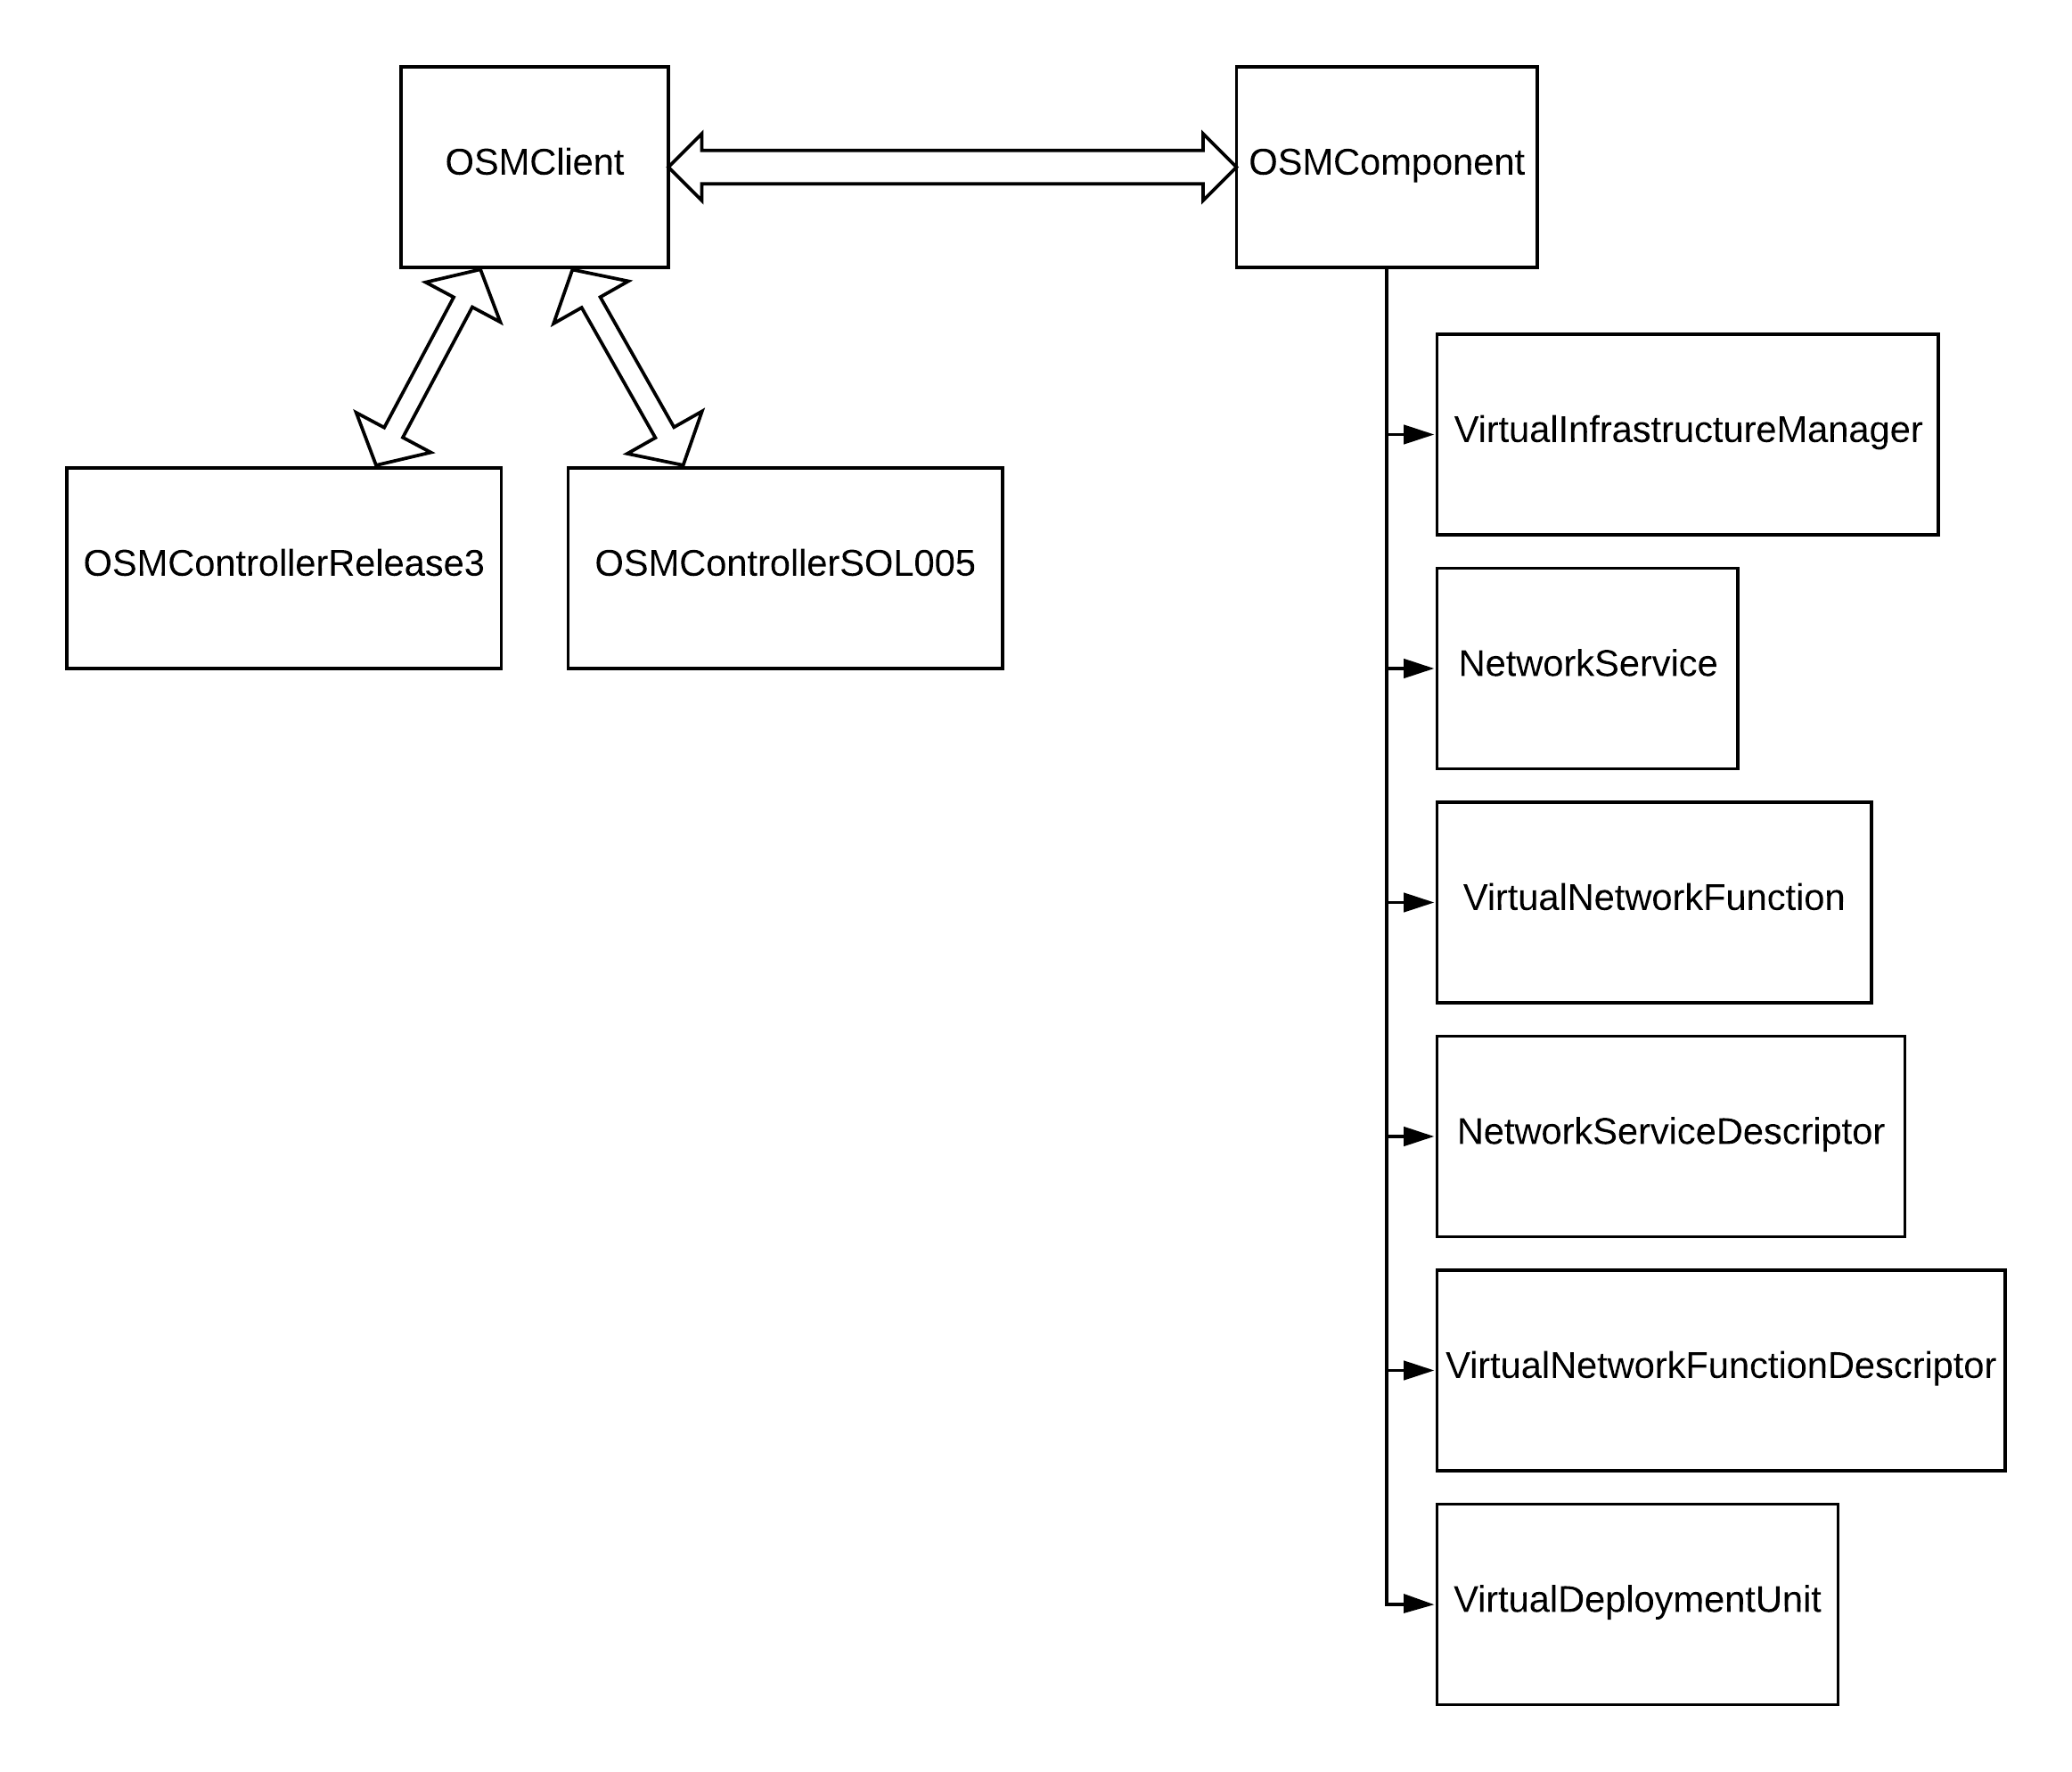
\includegraphics[width=0.8\linewidth]{imagenes/OSMClient}
	\caption{Estructura de clases de J-OSMClient}
	\label{fig:osmclient}
\end{figure}

En la figura \ref{fig:osmclient} se puede ver un esquema detallado de la jerarquía de clases. Se aprecia como OSMClient interactúa directamente con ambos \textit{controllers} para establecer la comunicación con ambas versiones de OSM.


\section{J-ONOS Client}
\label{sec:onosclient}

\begin{figure}[!ht]
	\centering
	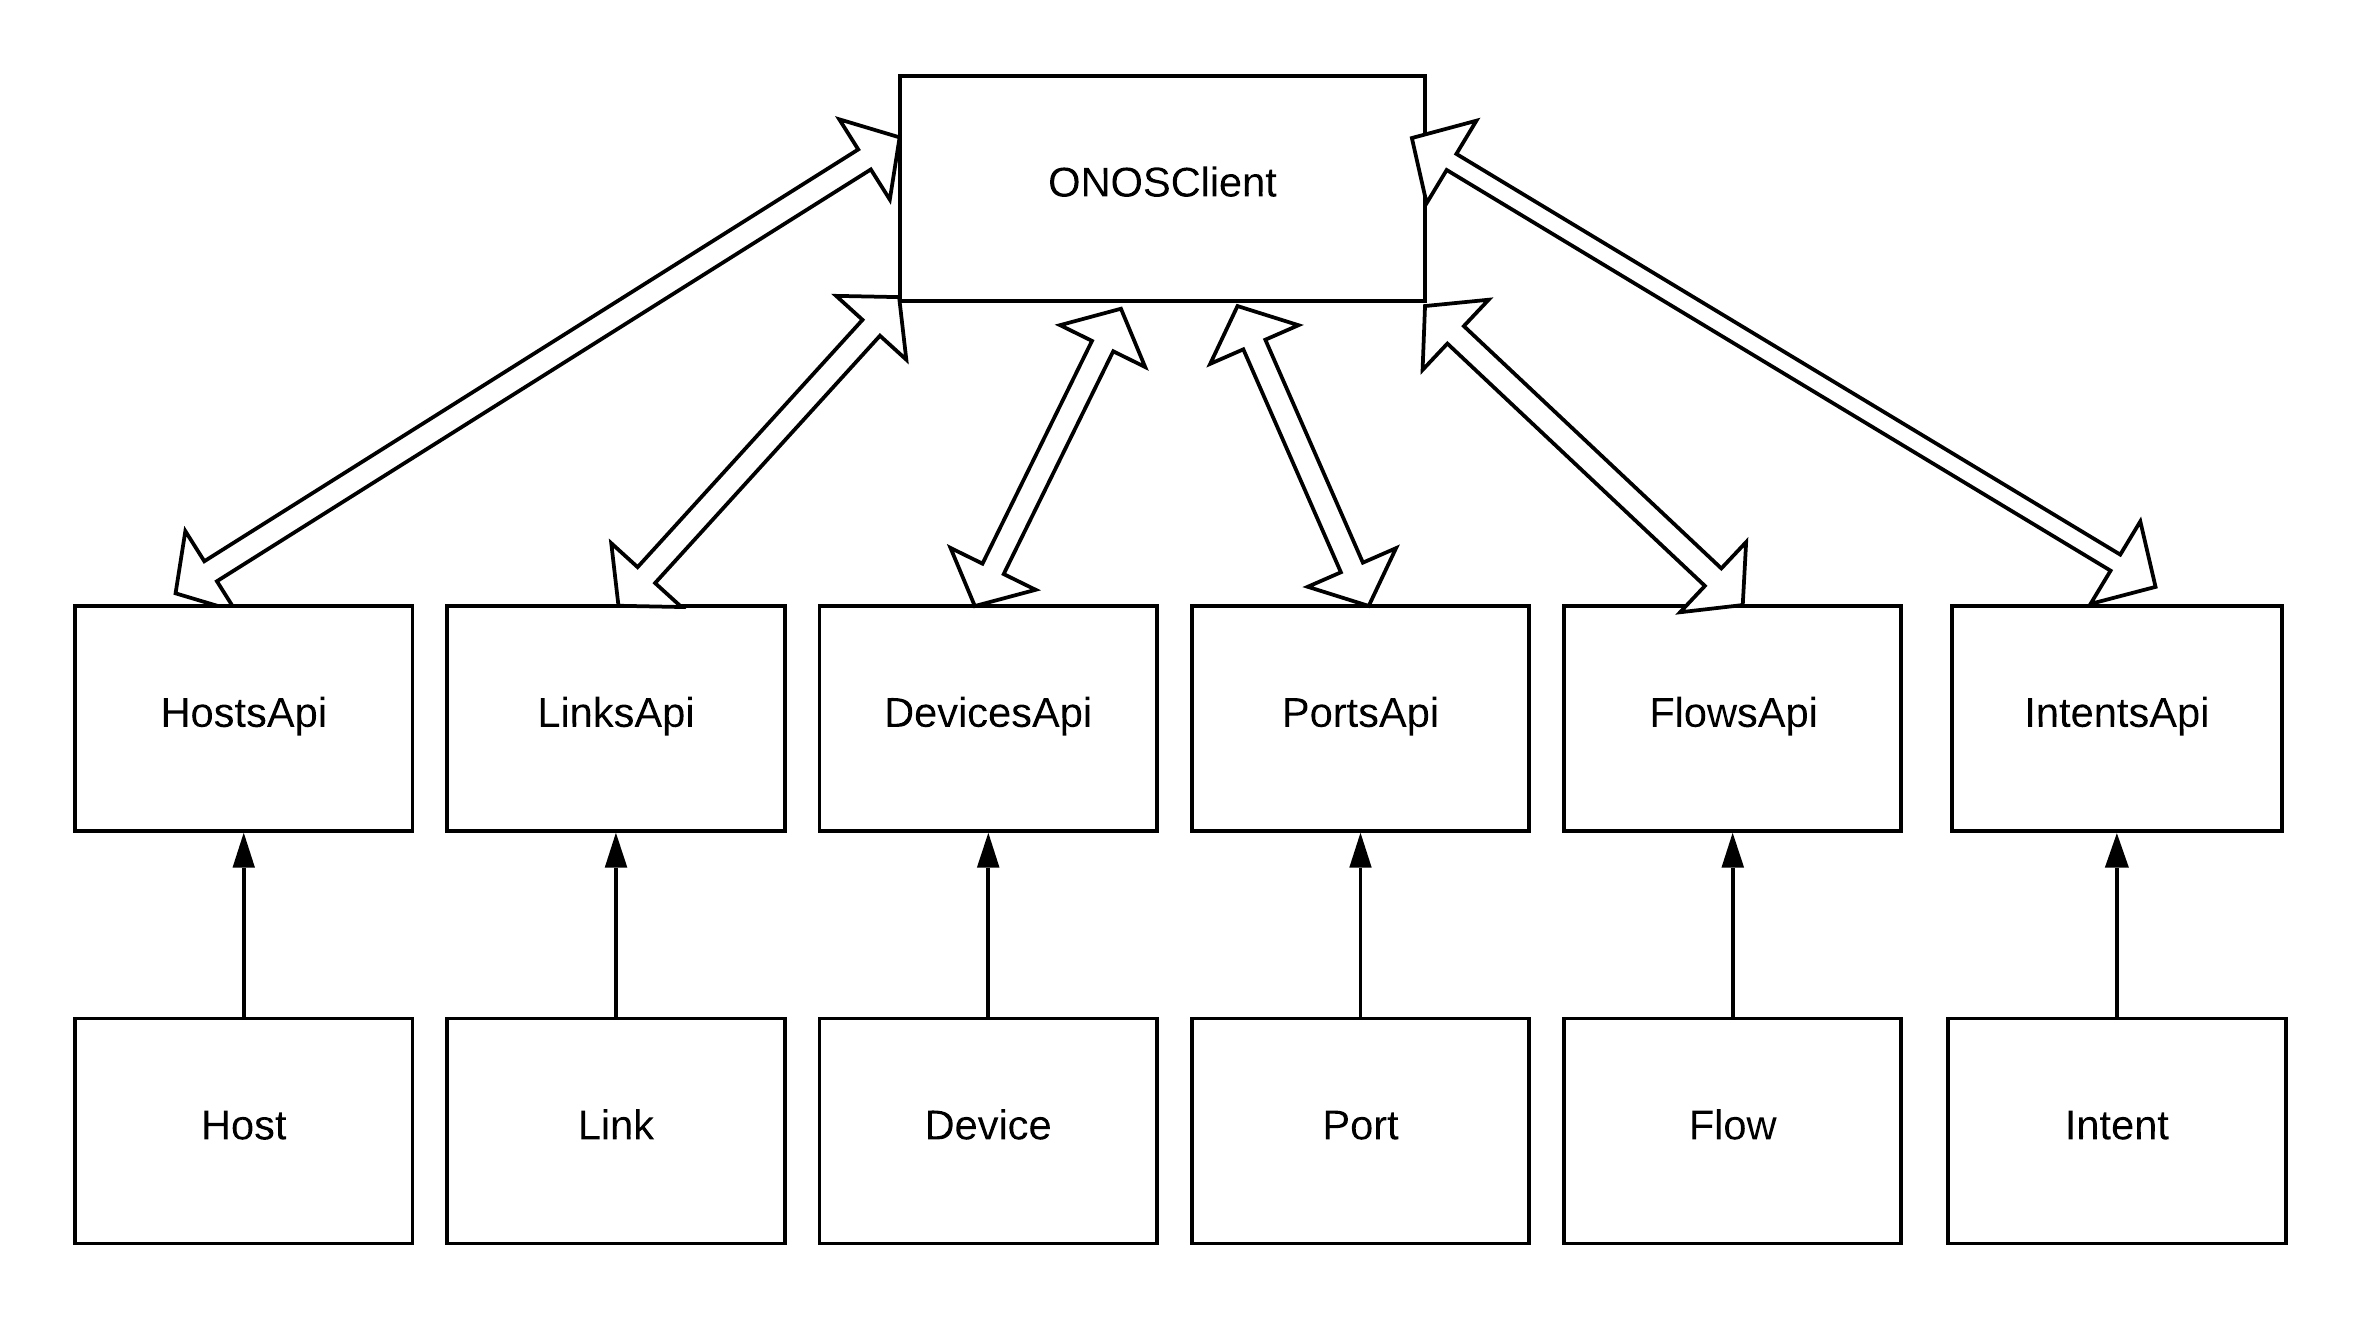
\includegraphics[width=0.8\linewidth]{imagenes/ONOSClient}
	\caption{Estructura de clases de ONOSClient}
	\label{fig:onosclient}
\end{figure}


\section{J-OpenStack Client}
\label{sec:openstackclient}

\begin{figure}[!ht]
	\centering
	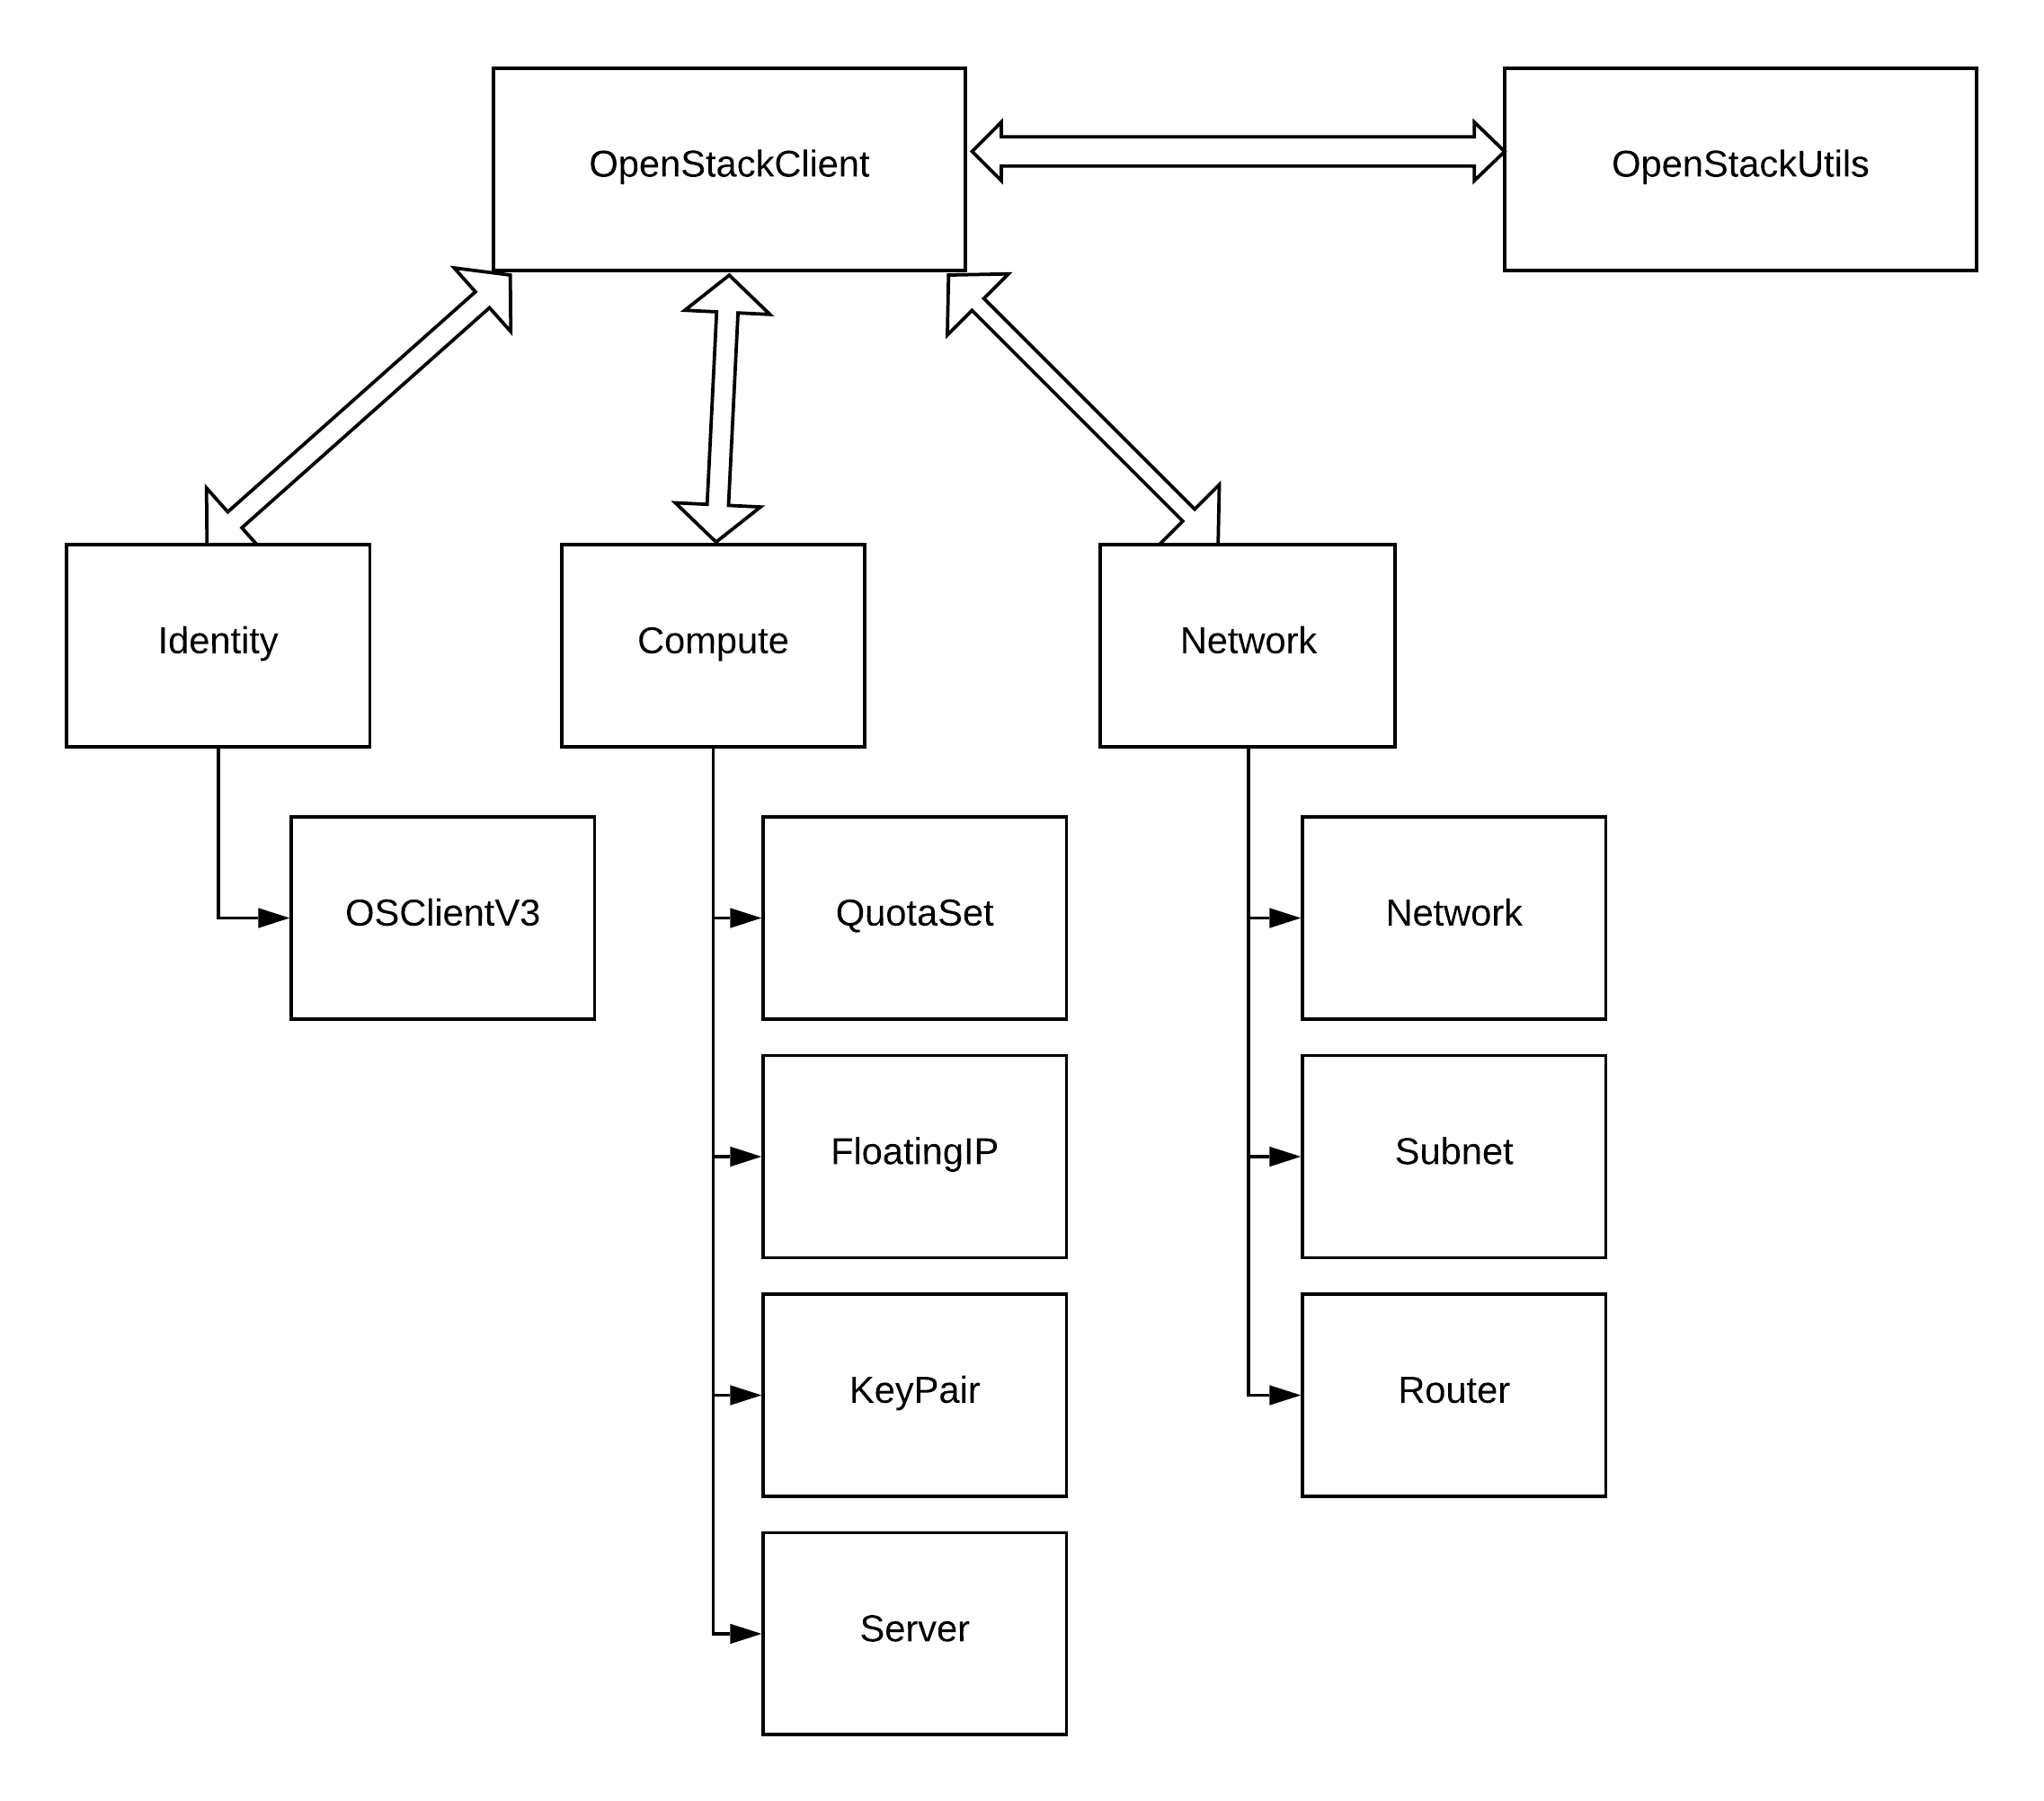
\includegraphics[width=0.8\linewidth]{imagenes/OpenStackClient}
	\caption{Estructura de clases de OpenStackClient}
	\label{fig:openstackclient}
\end{figure}

\section{Net2Plan: NFV Management Plugin}
\label{sec:nfvplugin}

Para llevar a cabo este proyecto, era necesario integrar las APIs mencionadas anteriormente con una herramienta que tenga funcionalidad de planificación de redes. Por ello, se ha desarrollado una extensión de Net2Plan basada en el plugin Network Design.


\begin{figure}[!ht]
	\centering
	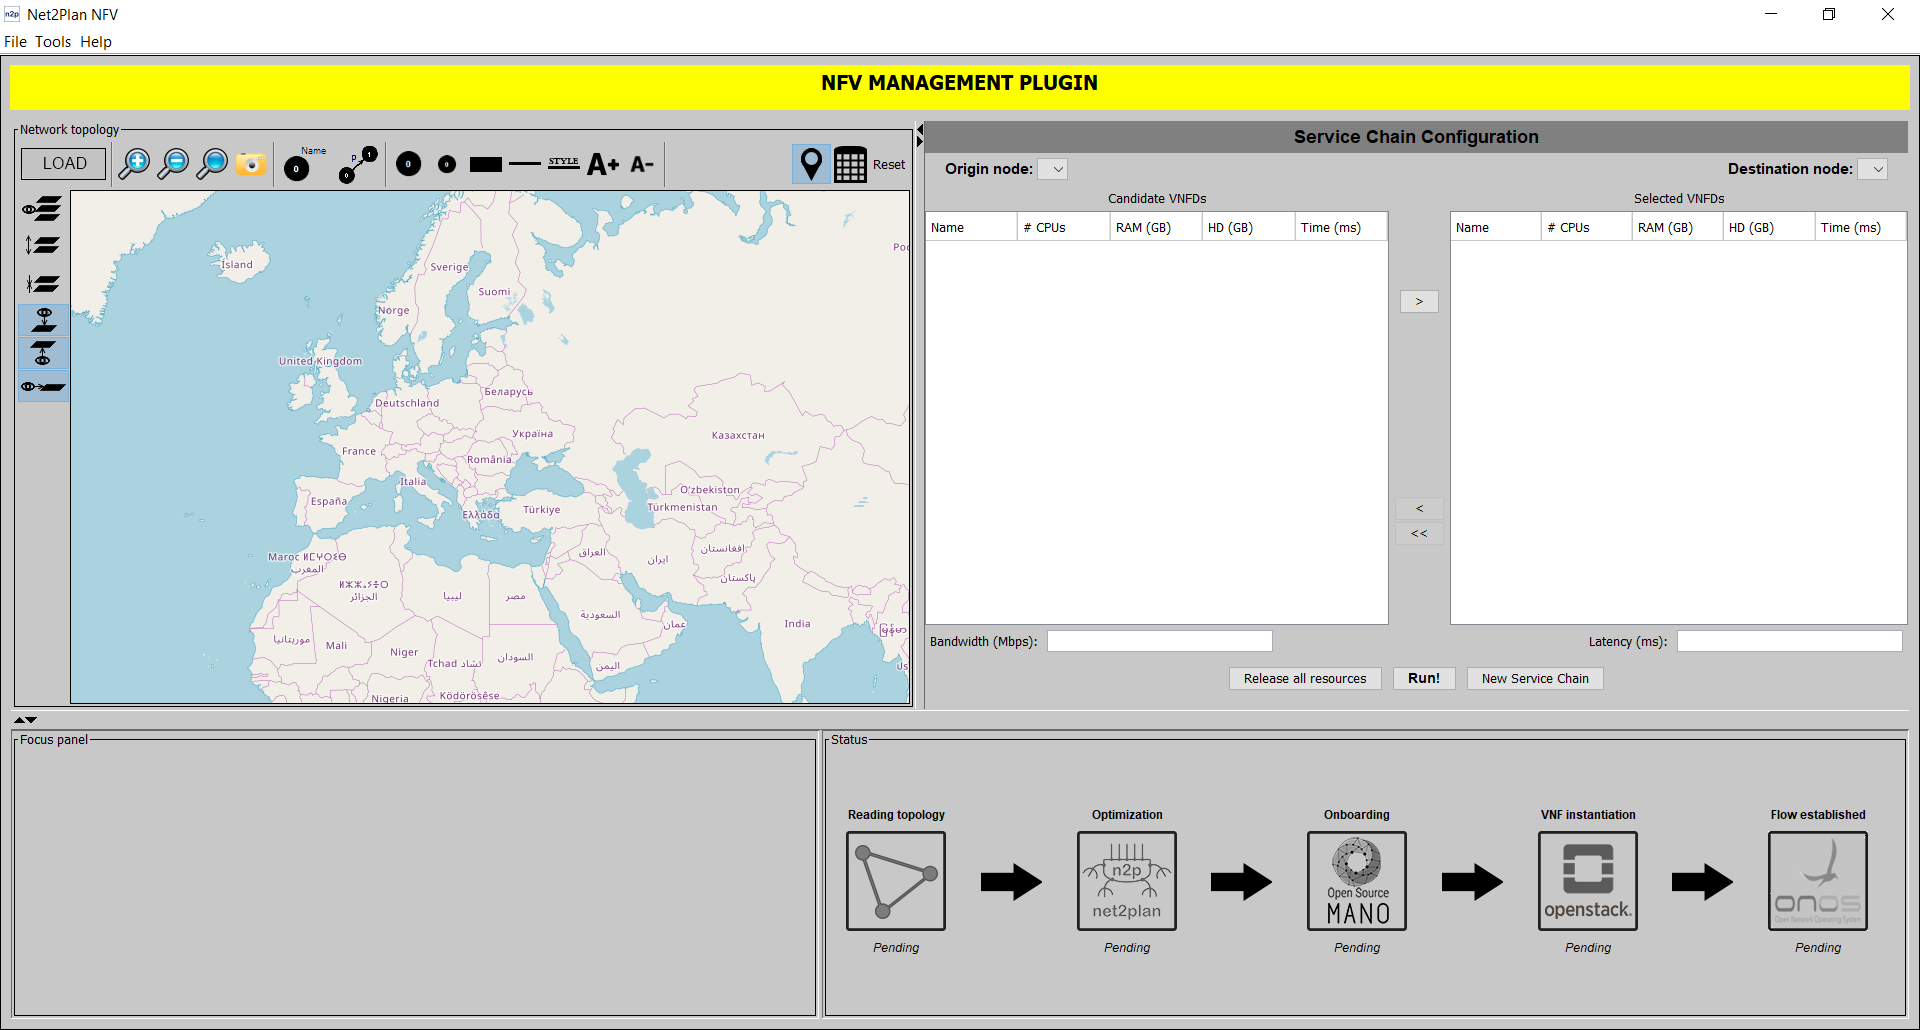
\includegraphics[width=0.8\linewidth]{imagenes/nfvplugin_dashboard}
	\caption{Interfaz gráfica del Plugin NFV-Management}
	\label{fig:nfvplugindash}
\end{figure}

Así mismo, en la figura \ref{fig:nfvplugindash} se puede observar la interfaz gráfica del Plugin NFV-Management, la cual está dividida en diferentes secciones:

\begin{itemize}
	\item Arriba a la izquierda se encuentra el \textit{TopologyPanel}, que se encarga de dibujar la topología deseada. Esta funcionalidad es heredada del \textit{Plugin Network Design} de Net2Plan.
	
	\item Arriba a la derecha se encuentra el \textit{OSMPanel}, que se encarga de obtener información sobre los distintos NSD que se encuentran disponibles en OSM y mostrarla al usuario de una manera amigable, informándole de que recursos (HD, RAM, CPU) son necesarios para su instanciación en un VIM.
	
	\item Abajo a la izquierda se encuentra el \textit{FocusPanel}, que se encarga de mostrar información detallada de un elemento en concreto cuando se selecciona. Dicha funcionalidad es heredada del \textit{Plugin Network Design} de Net2Plan.
	
	\item Abajo a la derecha se encuentra el \textit{ServiceChainPanel}.
\end{itemize}




\cleardoublepage